Le rotor d'un hélicoptère est la partie mobile qui va entraîner la rotation de ses pales.

\textbf{Étude de la vitesse de rotation du rotor}

La vitesse de rotation du moteur, notée $\omega$ et exprimée en $\mathrm{rad}\cdot\mathrm{s}^{-1}$, est solution de l'équation différentielle suivante :
\[y' = - 0,028y + 18,48.\]

\begin{enumerate}[start = 3]
	\item Montrer que la fonction $\omega$ définie sur $[0~;~+\infty[$ par
	\[\omega(t) = - 660 \e^{-0,028t} + 660\]

	est la solution de cette équation différentielle qui vérifie la condition initiale $\omega(0) = 0$.

	\item Déterminer $\displaystyle\lim_{t \to + \infty} \omega(t)$.
	Cette limite correspond à la valeur maximale de la vitesse de rotation du moteur.
\end{enumerate}

Un système mécanique fixe la vitesse de rotation du rotor par rapport à celle du moteur :
\[\omega_{\text{rotor}} = \dfrac{1}{20}\omega_{\text{moteur}}.\]

On donne l'évolution de la vitesse de rotation du rotor en fonction du temps dans le \textbf{document \no 2}.

\medskip

\begin{tblr}{colspec=X[c],hlines, vlines}
	%Début tikz
	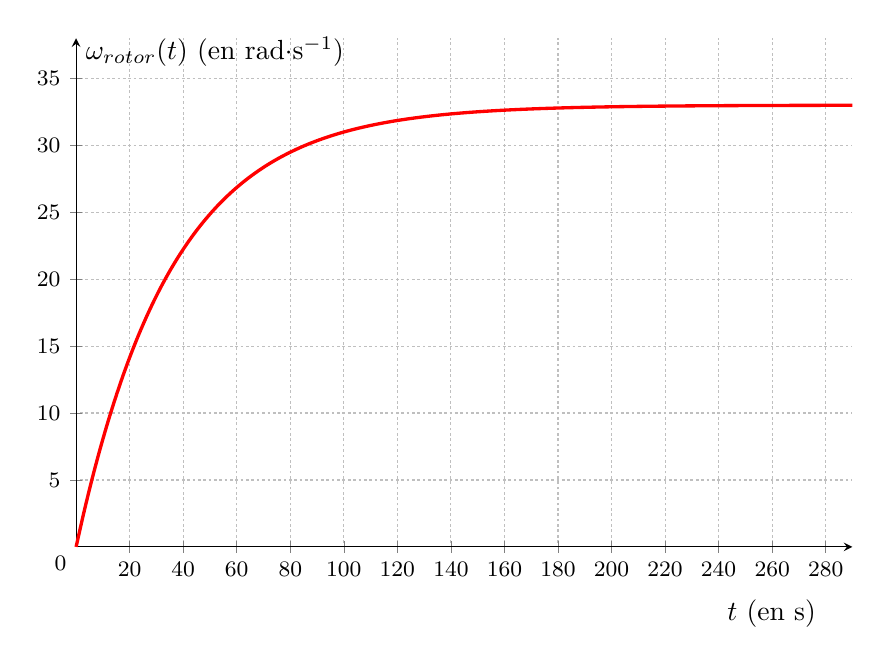
\begin{tikzpicture}%compiler avec pgfplots
		\begin{axis}[/pgf/number format/.cd, use comma,
			x={0.34mm}, y={1.7mm},
			xmin =0 , xmax = 290,
			ymin =0 , ymax = 38,
			xtick distance = 20,
			ytick distance = 5,
			tick label style={font=\footnotesize},
			clip=false,grid style={dash pattern=on 0.34mm off 0.34mm,dash phase=0.17mm},
			grid=major, axis lines =center]
			\addplot [line width=1.2pt,color=red,smooth,samples=100,domain= 0:290 ]{-33*exp(-0.028*x)+33};
			\node[below left] at (axis cs: 0,0) {{\footnotesize 0}};
			\node[anchor= west] at(axis cs: 0,37) {$\omega_{\text{rotor}}(t)$ (en rad$\cdot$s$^{-1}$)};
			\node[anchor= east] at(axis cs: 280,-5) {$t$ (en s)};
		\end{axis}
	\end{tikzpicture}
	%Fin tikz
%%%%Début pstricks
%	\psset{xunit=0.05cm,yunit=0.2cm,arrowsize=2pt 3}
%	\begin{pspicture}(-20,-4)(290,40)
%		\psaxes[linewidth=1.25pt,Dx=20,Dy=5,labelFontSize=\scriptstyle] {->}(0,0)(290,40)
%		\multido{\n=0+20}{15}{\psline[linewidth=0.25pt](\n,0)(\n,35)}
%		\multido{\n=0+5}{8}{\psline[linewidth=0.25pt](0,\n)(290,\n)}
%		\uput[u](270,0){\small $t$ (en s)}\uput[r](0,38){\small $\omega_{\text{rotor}}(t)$ (en rad.s$^{-1}$)}
%		\psplot[plotpoints=2000,linewidth=1.25pt,linecolor=red]{0}{290}{33 1 2.71828 0.028 x mul neg exp sub mul}
%	\end{pspicture}
%%%%Fin pstricks
	\\
	\textbf{Document \no 2 : évolution de la vitesse de rotation du rotor en fonction du temps}
\end{tblr}

\begin{enumerate}[resume]
	\item Donner la vitesse maximale de rotation du rotor.
\end{enumerate}

Le rayon des pales, noté $R$, vaut 5 mètres.
\begin{enumerate}[resume]
	\item En déduire la valeur de la vitesse maximale de l'extrémité de la pale.
\end{enumerate}

La vitesse du son dans l'air vaut 344 m·s$^{-1}$ pour une température de 20~\degres C.

Pour des raisons de sécurité, la vitesse instantanée à l'extrémité des pales doit rester inférieure à la vitesse du son dans l'air.
\begin{enumerate}[resume]
	\item Conclure sur le respect des règles de sécurité.
\end{enumerate}

\bigskip
